\chapter{Исследовательская часть}

Для работы с разработанным загружаемым модулем ядра была использована электронная вычислительная машина, обладающая следующими характеристиками:
\begin{itemize}
	\item операционная система Manjaro Linux x86\_64~\cite{manjaro};
	\item процессор Intel i7-10510U 4.900 ГГц~\cite{cpu};
	\item оперативная память DDR4, 2400 МГц, 8 ГБ~\cite{ram}.
\end{itemize}

Для проверки работы разработанного программного обеспечения был реализован загружаемый модуль ядра exp\_md, осуществляющий создание и уничтожение SLAB-кэшей, а также выделение и освобождение объектов в SLAB-кэшах.
Исходный код загружаемого модуля ядра exp\_md представлен в приложении Б.

Во время загрузки загружаемого модуля ядра exp\_md в SLAB-кэше выделяются объекты следующих структур:
\begin{itemize}
	\item struct s1,
	\item struct s2,
	\item struct s3.
\end{itemize}

Объявления данных структур представлены в листинге~\ref{test_structs}.
\begin{figure}[H]
	\begin{lstlisting}[label=test_structs,caption=Структуры для проведения проверки работы загружаемого модуля ядра для мониторинга SLAB-кэша,language=Caml]
struct s1
{
	int a;
	char b;
	
	struct file arr[100];
};

struct s2
{
	int a;
	char b;
};

struct s3
{
	size_t a;
	size_t b;
	size_t c;
	size_t d;
	
	struct file f;
};
	\end{lstlisting}
\end{figure}

Для объектов выше описанных структур создаются SLAB-кэши s1\_cache, s2\_cache и s3\_cache соответственно.

На рисунках~\ref{exp1}~--~\ref{exp6} представлены данные об использовании SLAB-кэша во время инициализации загружаемого модуля ядра exp\_md.
\begin{figure}[H]
	\centering
	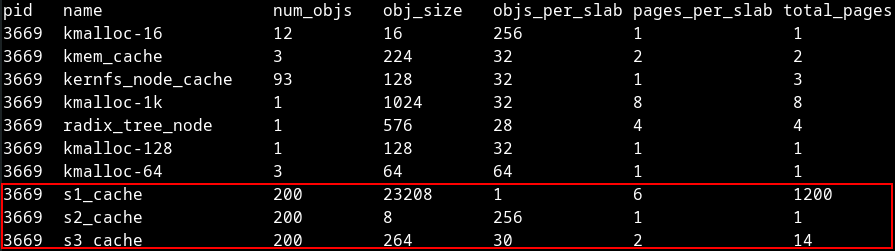
\includegraphics[width=\linewidth]{exp1}
	\caption{Данные об использовании SLAB-кэша после выделения 200 объектов структуры struct~s1, 200 объектов структуры struct~s2 и 200 объектов структуры struct~s3}
	\label{exp1}
\end{figure}
\begin{figure}[H]
	\centering
	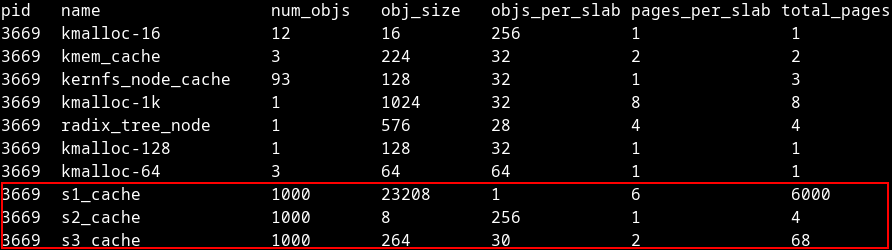
\includegraphics[width=\linewidth]{exp2}
	\caption{Данные об использовании SLAB-кэша после выделения 800 объектов структуры struct~s1, 800 объектов структуры struct~s2 и 800 объектов структуры struct~s3}
	\label{exp2}
\end{figure}
\begin{figure}[H]
	\centering
	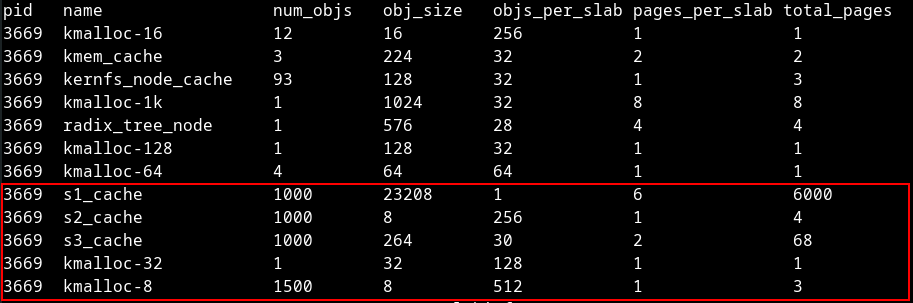
\includegraphics[width=\linewidth]{exp3}
	\caption{Данные об использовании SLAB-кэша после выделения 1500 объектов структуры struct~s2 с помощью системного вызова kmalloc}
	\label{exp3}
\end{figure}
\begin{figure}[H]
	\centering
	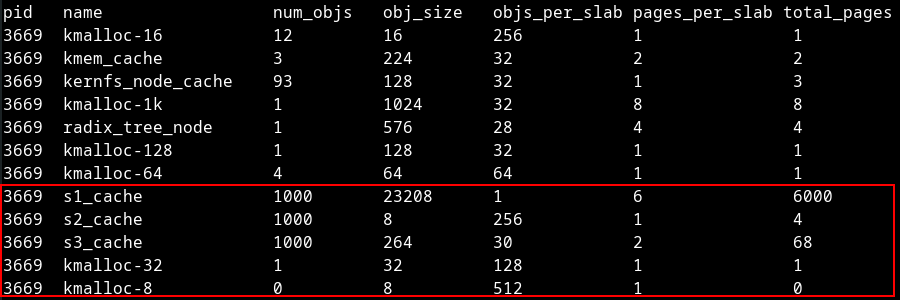
\includegraphics[width=\linewidth]{exp4}
	\caption{Данные об использовании SLAB-кэша после освобождения 1500 объектов структуры struct~s2 с помощью системного вызова kfree}
	\label{exp4}
\end{figure}
\begin{figure}[H]
	\centering
	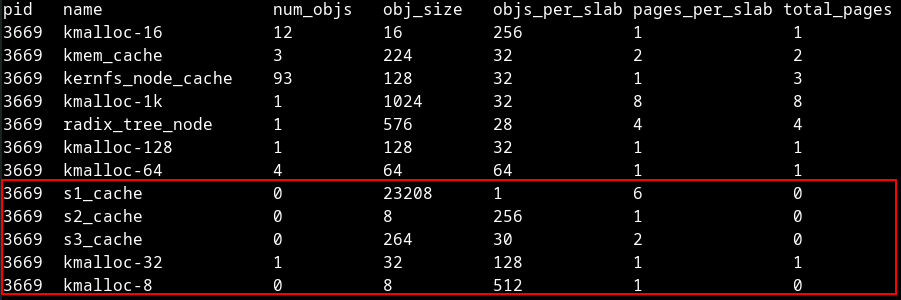
\includegraphics[width=\linewidth]{exp5}
	\caption{Данные об использовании SLAB-кэша после освобождения 1000 объектов структуры struct~s1, 1000 объектов структуры struct~s2 и 1000 объектов структуры struct~s3}
	\label{exp5}
\end{figure}
\begin{figure}[H]
	\centering
	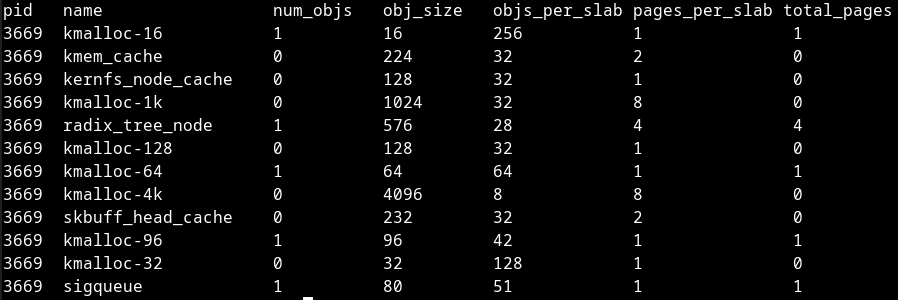
\includegraphics[width=\linewidth]{exp6}
	\caption{Данные об использовании SLAB-кэша после уничтожения кэшей s1\_cache, s2\_cache и s3\_cache}
	\label{exp6}
\end{figure}

\section{Вывод}

Была проведена проверка работы разработанного загружаемого модуля ядра для мониторинга использования SLAB-кэша процессами в операционной системе Linux.
Реализованный загружаемый модуль ядра работает исправно.

\clearpage
